\section{Approaching high densities: supercooled liquids and glasses}
%% \subsection{Mean-field picture}
%% The infinite dimensional limit $d \to \infty$.

%% \subsection{Random first-order transition theory}
%% Perturbation from mean-field in $1/d$.

%% \subsection{Alternative pictures in physical dimensions}
%% For $d \le 3$
%% \subsubsection{Frustration-limited domain theory}
%% \subsubsection{Dynamical theories}

It is widely reported that glass is actually liquid, and as evidence of this the thickness of old windows at the bottom is pointed to.
This is actually a matter of some dispute, but contains a grain of truth.
Pre-modern methods of creating window glass involved spinning molten glass on magma to flatten it out.
Centrifugal forces caused the glass to be thicker on the outer disk, so panes of glass would always be heavier in one direction%
\marginfootnote{And personally, if I were setting an uneven pane of glass I would place the heavy part at the bottom.}.

To a soft matter physicist glass is a broader term, referring to a wide class of materials while the window glass of common parlance is referred to by its chemical name \emph{silicate}.
This class of materials share many features of being disordered etc \cite{?} although in some sense they are connected by what they do \emph{not} do: which is flow on human timescales.
When I refer to `glass' I will be using it in this broad technical sense of a state of matter.
Some examples besides silicate:
\begin{itemize}
\item Most of the ice in the universe exists in an amorphous state in comets \cite{?}
\item Ceramics
\item Plastics: amorphous polymers
\end{itemize}
Of more abstract nature which could be called glassy though they are not materials
\begin{itemize}
\item Gels: super glasses, liquid like bit plus a network/backbone which has glassy dynamics
\item Neural networks
\item Non-deterministic polynomial time (NP) problems
\end{itemize}
We will not be directly addressing the latter type of more abstract problems which could be considered glasses, although they are arguably related due to a similar underlying disorder.
We will be focusing on only the most rudimentary of glassy phenomenology: the dynamical arrest of liquids at high densities/low temperatures when crystallisation is avoided.
Especially as it manifests in hard spheres, which as discussed is the reference system of choice for simple liquids.

So what do we mean by dynamical arrest.
Typically we can look at one of two (related) quantities: viscosity or relaxation time.
Viscosity measures how resistant the thing is to flow, while relaxation time measures the typical microscopic time for things to move around i.e.\ liquid like behaviour.
As a practical definition, a glass is defined in the lab as any material for which the relaxation time exceeds 100\ce{s}: this point is called the experimental glass transition.
This is somewhat arbitrary, although the location of the glass transition point is not particularly sensitive to where you set the threshold because of how rapidly the viscosity/times are increasing around there.
\todo{Need: Angell plot, fragile vs strong}

Personally, the observation that got me interested in the field is the entropy argument.
If one compares the difference between the entropy of the crystal and the glass, and extrapolates wildly one expects there to be a point where the glass has a lower entropy than the crystal.
This is not very meaningful by itself, as we have already established by discussing the crystal vibrational entropy can be quite subtle so it is possible for the liquid to have a lower vibrational entropy.
However, if one corrects this with more modern techniques to measure just the entropy corresponding to non-trivial motion we see that there is a point where the configurational (i.e.\ not purely vibrational) entropy vanishes: this would imply the system is frozen in a single configuration.
Such a point would define a transition to a genuine thermodynamic phase, an ideal glass.
\todo{Plots of configurational entropy}

A diverging timescale necessarily requires a diverging point-to-set length scale and a vanishing configurational entropy, a proof given in \cite{?}.
This must trivially occur at the very least $T=0\si{K}$ where relaxation timescales diverges, however much like the lack of a phase transition in the Ising model in $d=1$ this is not a true thermodynamic phase transition because it cannot be crossed.
Recent numerical evidence suggests that a model glassformer in $d=2$ does not show a transition, also vanishing at $T=0\si{K}$ \cite{Berthier?}.
So the central question of glass is what happens in $d=3$, is there a vanishing configurational entropy at a finite $T > 0$ with an accompanying thermodynamic glass transition?
In mean-field, formally in the limit of infinite spatial dimensions $d \to \infty$, the hard sphere system has been shown to have a true transition, however the critical dimensions are unknown so it is unclear what happens in $d=3$ \cite{Parisi,Zamboni,Charbonneau,Kurchan,?,?}.

\todo{Jamming: how does it relate to glass}

\subsection{Phenomenology: notes from Tarjus}

Overview of the glass transition.
Salient features: why hard, interesting, unique.

What is a glass?
Frozen in a (apparently) disordered state.
All sorts of glasses, structural, spin, orientational, electron, vortex.
Glasses formed by liquids, colloidal suspensions and polymers: traditional structural glasses.
Solid: doesn't flow on observational time, resists small/infinitesimal shear (acts like solid).
Amorphous, apparently amorphous: no periodic arrangement like in crystal.
Homogeneous makes useful for technology: useful for e.g.\ optical properties.

Hard glasses: high elastic constants.
Colloidal suspensions: soft matter version, small elastic constants.
Same phenomenology though.

Cooling a liquid.
Take thermodynamic quantity (e.g.\ volume, entropy, enthalpy): usually crystallise.
(Picture)
First-order transition bypassed by quick cooling.
Enter supercooled liquid phase.
No longer equilibrates/relax/flows, call it a glass: occurs at glass transition.
Glass is a solid for all practical purposes.

SC liquid: same characteristics as at equilibrium.
Independent of preparation: loses memory of initial preparation.
Measureable properties have time translational invariance/are stationary.
Time independence of all observables, i.e.\
\begin{equation}
  \langle A(t) \rangle = \langle A \rangle
\end{equation}
including correlation functions e.g.\
\begin{equation}
  \langle A(t) A(t') \rangle = \langle A(0) A(t - t') \rangle
\end{equation}
(equation for stationary)
Fluctuation-dissipation theorems.
Linear response regime: response to perturbation related to correlation function (spontaneous fluctuations).
\begin{equation}
  \chi_A (t, t')
  =
  - \beta \Theta(t - t')
  \frac{d}{dt}
  \left(
  \bigg\langle
  (A(t) - \langle A \rangle)
  (A(0) - \langle A \rangle)
  \bigg\rangle
  \right)
\end{equation}

Distinguished from glass which has dependence on preparation history, hysteresis/memory effect of heating the system (will not follow exactly the same curve until - back to the equilibrium supercooled structure), aging: averages (including correlations) evolve in time.

The glass transition itself is not a ``transition'' in the thermodynamic sense; there is no.
It's really a kind of impatience transition; the glass transition for a human would be different to the glass transition for a demigod/ent.
It's still a relatively robust measurement, because of the superarrhenius scaling (sc-l for pedestrians).

No glass from noble gases; too high propensity for first order transition.

Below melting, the crystal is the state lowest in free energy so strictly metastable.
Though not strictly an equilibrium state, we can think about it as such.
Hard spheres have particular propensity to crystallise at very high densities, so typically polydispersity is introduced to frustrate crystals favouring amorphous structures.

A plethora of questions related to the out-of-equilibrium properties.
\begin{enumerate}
\item Properties of out of equilibrium glass phase: very important questions for material science. Low temperature anomalies, aging behaviour, nonlinear rheology  plasticity.
\item Relation between glass and jamming. Jamming=zero temperature, out of equilibrium, infinite pressure.
\item How to avoid crystallisation.
\end{enumerate}



\subsection{What is there to be explained about the glass transition?}

Understand prpoerties of the supercooled liquid, that distinguish it from ordinary liquids (dynamically).

Remarkable dynamic range: observed change over 16 orders of magnitude.
Arrhenius plot.
Experiments: dynamic light scattering.
\begin{equation}
  \langle \delta A(0) \delta A(t) \rangle
  \to \tau_{relax}
\end{equation}
Decay of function gives timescale.
Angell plot (1984?): rescale by Tg and classify different systems.
Strong: Arrhenius, fragile: super-arrhenius (this naming system is odd: it has nothing to do with their mechanical properties)

Assume single fundamental process in relaxation: e.g.\ breaking a chemical bond.
Then barrier constant leads to Arrhenius law.
\begin{equation}
  \tau \sim \tau_0 e^{\frac{\Delta U}{T}}
\end{equation}
(could be free energy)
Interactions in soft matter are typically van der Waals, very weak, so to build large activation energy lots of particles must be contributing.
Super Arrhenius behaviour must arise from collective behaviour.
Collective behaviour: many-body effects requires many-body correlations.

Some systems are Arrhenius: particularly in hard matter systems where interactions are stronger.
E.g.\ Silicate: covalent bonds, so barrier is that required to break a bond.

Some modification is required for hard particle systems: instead of 2d phase diagram (density-temperature) we have 1d (density).
Hard spheres highly fragile: more collective effects.
Easier to see that collective effects: activation barriers must be strictly entropic, which is perhaps easier to argue for collective effects.

Phenomenological formula...

Relationship with viscosity.
Flowing/not flowing is captured by viscosity: viscous slowdown same as relaxation slowdown.
Slightly different notion.
Short times $t \ll \tau$: elastic system, long times $t \gg \tau$: viscosity.
Time barrier is relaxation time.
Elasticity, viscosity in Newtonian fluids: viscoelastic behaviour (Maxwell)
\begin{equation}
  \eta = G_\infty \tau_\mathrm{relax}
\end{equation}
high frequency shear modulus is elastic property.
Shear modulus increases by factor 2-5 times, is dwarfed by change in relaxation time.

No crystal: eutectic polymers

In conventional condensed matter physics dynamics is determined by structure.
For example, crystalline solids are fixed on a lattice so do not flow, whereas liquids are disordered and are thus able to flow.
Soft matter systems (e.g.\ gels, foams, glasses) do not neatly fall into this paradigm: their dynamics are often arrested whilst their structure remains highly disordered.

To illustrate the disentanglement between structure and dynamics we will take glasses as an example, because this will be the focus of our work.
A glass is obtained by supercooling a liquid causing its viscosity to increase dramatically.
Viscosity is equivalently measured by a timescale $\tau_\alpha$ for spatial correlations to decay.
This relaxation event should occur against some energy barrier $\Delta$, leading to the scaling relation
\begin{equation}\label{eq:angell}
  \tau_\alpha = \tau_0 \exp{\left(\frac{\Delta}{k_B T}\right)}
\end{equation}
for Boltzmann factor $k_B$, temperature $T$ and where $\tau_0$ is the timescale of vibrations (typically $\tau_0 \sim \mathcal{O}(1)$ps for atomic systems).
When $\tau_\alpha$ exceeds an experimentalist's patience (defined as 100s at temperature $T_g$ in the literature), it becomes impossible to properly equilibrate the liquid and we call it a glass.
On accessible timescales the glass will appear (macroscopically) solid, developing a bulk shear modulus etc, yet microscopically it remains disordered like a liquid. 

Naively we might expect $\Delta$ in \eqref{eq:angell} to be temperature independent, suggesting the \emph{Arrhenius} law:
\begin{equation}\label{eq:arrhenius}
  \log{\tau_\alpha} \propto 1/T.
\end{equation}
This works well for high temperature liquids but \emph{can} break down at low temperatures suggesting qualitatively new physics for supercooled liquids.
This is shown in Figure~\ref{fig:angell} where $\log{\tau_\alpha}$ is plotted against $1/T$ for selected molecular and model glassformers.
Silica is seen to increase according to \eqref{eq:arrhenius} even at low temperature; this is an example of a \emph{strong} glass which we are not interested in because the underlying physics is essentially that of a slow liquid.
We are instead interested in the deviations from \eqref{eq:arrhenius} displayed by the other systems shown in Figure~\ref{fig:angell}.
These so-called \emph{fragile} glassformers feature more dramatic increase in relaxation times than predicted by \eqref{eq:arrhenius}, meaning $\Delta$ itself increases with supercooling.
This work involves detailed microscopic calculation of energy landscapes in model glassformers, with the intent of determining the cause of increasing relaxation barriers in supercooled liquids.

Above we presented a brief description of glassy phenomenology for systems where temperature is the important state variable, although this need not be the case in general.
Hard spheres are widely used to model liquids, interacting by the pair potential
\begin{equation}\label{eq:hs-pair}
  V(r) = \left\{
  \begin{array}{lr}
    \infty & r \le \sigma \\
    0 & r > \sigma
  \end{array}
  \right.
\end{equation}
for hard sphere diameter $\sigma$. 
As molecules are typically repulsive at short-range, the hard sphere system serves as a useful reference potential from which molecular detail can be reincorporated through perturbation theories.
Hard sphere phenomenology is thus relevant for understanding a wide-range of simple liquids.
However, \eqref{eq:hs-pair} does not set an energy scale, so hard spheres are \emph{athermal} and thus pressure is more meaningful than temperature as a state variable~\cite{Berthier2009}.
Relaxation barriers in hard spheres are \emph{entropic} in nature, and display the same phenomenology as temperature driven fragile glassformers as seen in Figure~\ref{fig:angell} where a reduced pressure has been defined as
\begin{equation}\label{eq:reduced-P}
  Z = \frac{P}{\rho k_B T}
\end{equation}
where $\rho$ is the density of the fluid. This variable plays the role of $1/T$ for athermal systems, although this analogy is only approximate.


\subsection{Thermodynamic}

\begin{SCfigure}
  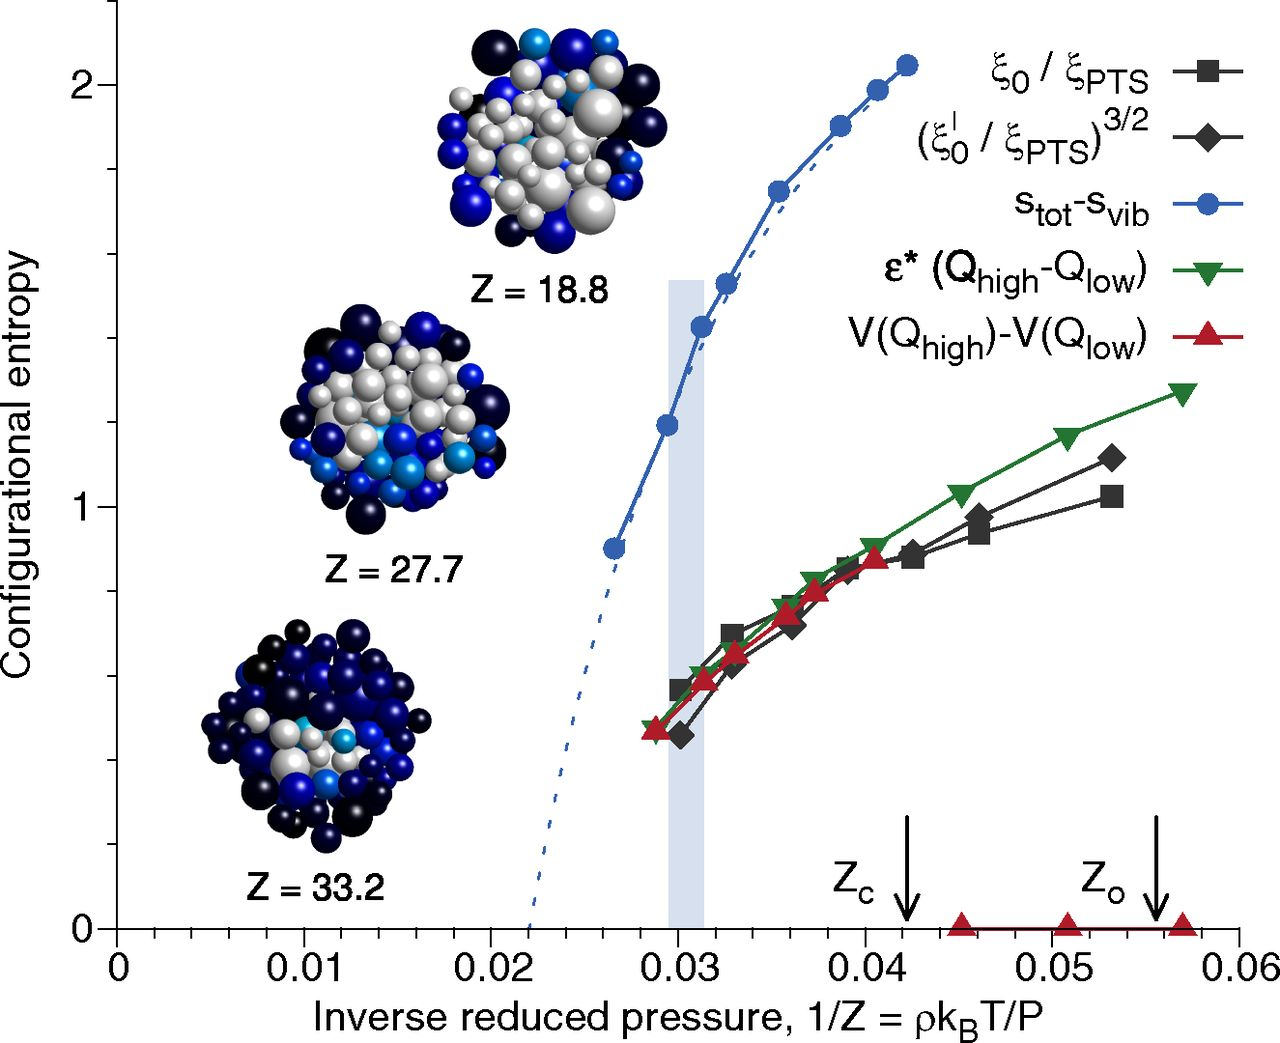
\includegraphics[width=\linewidth,outer]{swap-Sconf}
  \caption[Configurational entropy in hard spheres from Monte-Carlo simulations]{
    Configurational entropy.
    Reproduced from Ref.\ \cite{BerthierPNAS2017}.
  }
\end{SCfigure}

\subsection{Perspective: role of many-body correlations}

\hl{Derivatives of free energy reduce} to $g^{(2)}$,\hl{ emblematic of the conventional routes.
Absolute free energies require higher order correlation functions to appear.}
\todo{Talk about this. Also: entropy route.}

FMT already provides an easy route to obtaining correlation functions in Fourier space, as was demonstrated in the original papers \cite{RosenfeldPRL1989,RosenfeldJCP1990} and we will summarise below.
Applying the convolution theorem allows the Fourier transform of \eqref{eq:fmt-direct-correlations-uniform-density} to be written rather succinctly as
\begin{equation}
  \tilde{c}^{(n)}(\vec{k}^n)
  =
  - \sum_{\alpha_1, \alpha_2, \cdots, \alpha_n}
  \partial^n_{\alpha_1, \alpha_2, \cdots, \alpha_n} \beta f^\mathrm{ex} \;
  \left( \prod_{i=1}^n \widetilde{\omega}_{\alpha_i}(\vec{k}_i) \right)
  \delta(\vec{k}_1 + \vec{k}_2 + \cdots + \vec{k}_n).
\end{equation}
The delta function enforces the `ring' condition $\sum_{i=1}^n \vec{k}_i = 0$ which emerges from translational symmetry of the weight functions, reducing the dimensionality of the domain by $d$.
A further $d(d-1)/2$ degrees of freedom%
\marginfootnote{This many degrees of freedom can be removed for general $n \ge d$, but we expect fewer for $n < d$.
  For example, $n=2$ arrangements (a dimer) are isomorphic to a line so they possess $d-1$ rotational degrees of freedom.}
can be removed by exploiting rotational symmetry.
